% ****** Start of file apssamp.tex ******
%
%   This file is part of the APS files in the REVTeX 4.2 distribution.
%   Version 4.2a of REVTeX, December 2014
%
%   Copyright (c) 2014 The American Physical Society.
%
%   See the REVTeX 4 README file for restrictions and more information.
%
% TeX'ing this file requires that you have AMS-LaTeX 2.0 installed
% as well as the rest of the prerequisites for REVTeX 4.2
%
% See the REVTeX 4 README file
% It also requires running BibTeX. The commands are as follows:
%
%  1)  latex apssamp.tex
%  2)  bibtex apssamp
%  3)  latex apssamp.tex
%  4)  latex apssamp.tex
%
\documentclass[superscriptaddress,unsortedaddress,
%runinaddress,
%frontmatterverbose, 
%preprint,
%preprintnumbers,
%nofootinbib,
%nobibnotes,
%bibnotes,
 amsmath,amssymb,
 aps,
%pra,
%prb,
%rmp,
%prstab,
%prstper,
%floatfix,
]{revtex4-2}

\usepackage{graphicx}% Include figure files
\usepackage{dcolumn}% Align table columns on decimal point
\usepackage{bm}% bold math
\usepackage{physics}
\usepackage{lipsum}
\usepackage{subfig}
% \usepackage{braket}

%\newcommand\abs[1]{\left|#1\right|}
%\newcommand\bra[1]{\left| #1 \right \rangle}
%\newcommand\ket[1]{\left \langle #1 \right |}

\begin{document}


\title{Predicting Solid State Qubit Candidates}

\author{Oliver Lerstøl Hebnes}
\affiliation{Department of Physics and Center for Computing in Science Education, University of Oslo, N-0316 Oslo, Norway}
\author{Marianne Etzelm\"uller Bathen}
\affiliation{Advanced Power Semiconductor Laboratory, ETH Zürich, 8092  Zürich,  Switzerland}
\affiliation{Department of Physics and Center for Materials Science and Nanotechnology, University of Oslo, N-0316 Oslo, Norway}
\author{Øyvind Sigmundson Schøyen}
\affiliation{Department of Physics and Center for Computing in Science Education, University of Oslo, N-0316 Oslo, Norway}
\author{Sebastian G. Winther-Larsen}
\affiliation{Department of Physics and Center for Computing in Science Education, University of Oslo, N-0316 Oslo, Norway}
\author{Morten Hjorth-Jensen}
\affiliation{Facility for Rare Ion Beams and Department of Physics and Astronomy, Michigan State University, East Lansing, MI 48824, USA}
\affiliation{Department of Physics and Center for Computing in Science Education, University of Oslo, N-0316 Oslo, Norway}
\author{Lasse Vines}
\affiliation{Department of Physics and Center for Materials Science and Nanotechnology, University of Oslo, N-0316 Oslo, Norway}

\begin{abstract}

Semiconductor materials provide a compelling platform for quantum
technology, and a vast amount of materials and their properties can be
found in high-throughput databases.  However, filtering among these
materials in order to find novel candidates for quantum technology is
a challenge. Therefore, we provide a framework for the automatic
discovery of promising solid-state material hosts using machine
learning methods.

%Main message 1: develop methodology for data mining and machine learning for materials properties 
We have developed data extraction tools for numerous material science
databases, and constructed over $4800$ physics-informed features for a
dataset consisting of more than $25000$ materials.  Furthermore, we
have developed and implemented three data mining approaches, termed
\textit{the Ferrenti approach}, \textit{the augmented Ferrenti
  approach} and \textit{the insightful approach} for defining three
distinct training sets for the supervised machine learning algorithms
logistic regression, decision tree, random forest and gradient boost
to be trained on.

% Main message 2: Use method to propose new materials that are promising quantum hosts 
We find a lack of consistent results for the Ferrenti approach and the
augmented Ferrenti approach due to an overly broad formulation of the
training set, whereas the restrictions set in the insightful approach
proved suitable. All models agreed on $214$ predicted candidates, with
examples such as ZnGeP$_2$, MgSe, CdS, BP, BC$_2$N, BP, Ge, GeC, InP,
and InAs. All approaches and all models agreed on a subset of $47$
eligible candidates of $8$ elemental, $29$ binary, and $10$ tertiary
compounds.

\end{abstract}

\pacs{02.70.Ss, 31.15.A-, 31.15.bw, 71.15.-m, 73.21.La}




\maketitle

%Submit to npj Computational Materials

%Marianne: I have now structured the paper according to other papers in this journal 
%I think we can make a supplementary material if we see that we need it, it is quite common for the journal 

\section*{Introduction}%Oliver and Morten and Marianne (semiconductor portion)
To sustain the digital world’s increasing computational demand, alternatives to the classical computer must be explored. The quantum computer, together with the complementary quantum technologies of sensing and communication, is becoming a frontrunner in the race for solutions. 
Discuss recent benchmarks for quantum computing \cite{Arute_2019}. 

Limitations of quantum computing and technology building blocks. Drawbacks of superconductors. Semiconductors are a promising platform. Example of NV center in diamond \cite{Doherty_2013}. 

%From thesis - rewrite 
Unfortunately, there are substantial challenges associated with the modern quantum platforms simultaneously as the selection of quantum platforms are slim. The majority of discoveries of potential quantum platforms have so far happened by serendipity, and there is an urgent need for new and better materials that can escalate the effort for a sustainable future. 

The fourth science paradigm introduces the potential of targeted search for promising material systems to act as qubit hosts. 
Herein, we provide a framework for the automatic discovery of promising solid-state material hosts using machine learning methods. 
Initial database building similar to Ferrenti et al \cite{Ferrenti2020}. 

\begin{figure}
    \centering
    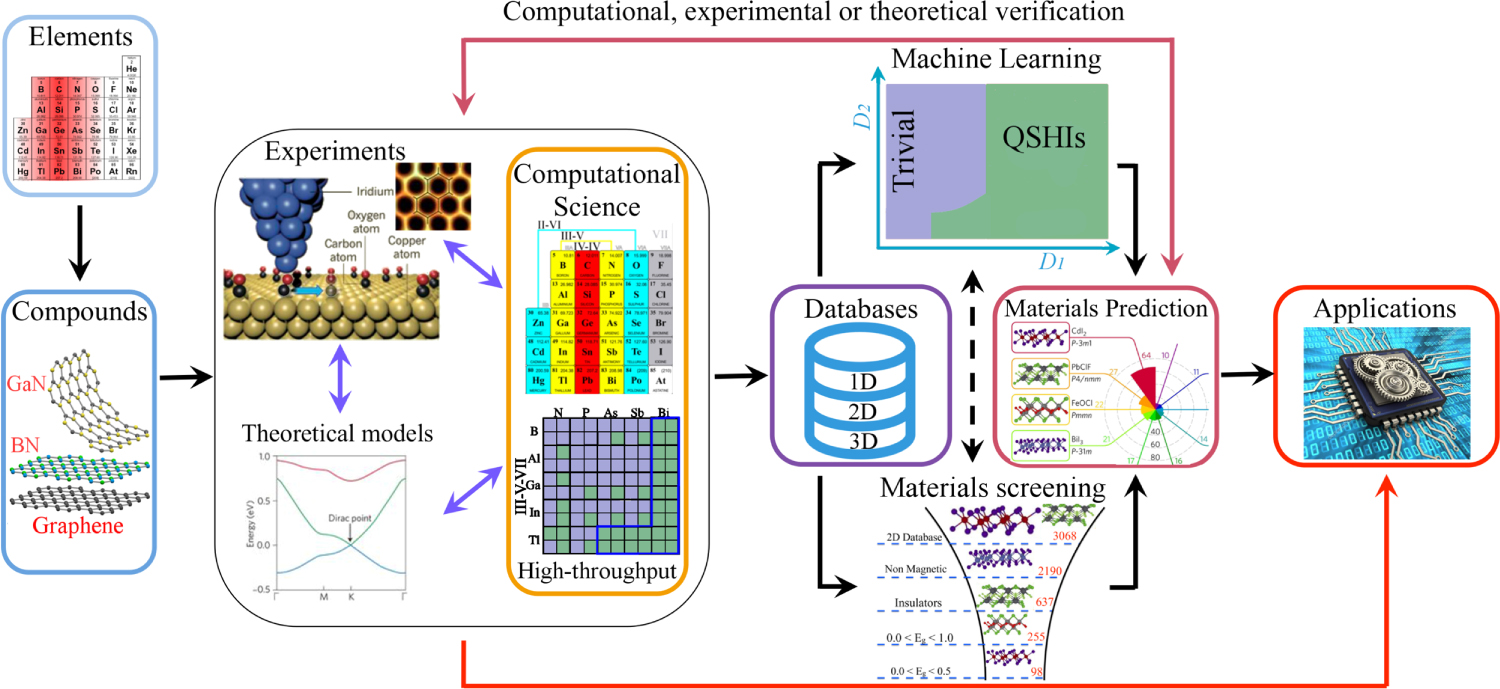
\includegraphics[width=\textwidth]{figures/ht-workflow.jpg}
    \caption{Placeholder for workflow. Morten: can you please add the other schematic figure we discussed as placeholder? Sebastian makes our own versions of these schematic figures (I can make some VESTA files with materials). }
    \label{fig:ht-workflow}
\end{figure}

\section*{Theoretical Background and Experimental Data} 
%Subsections are potential topics, not necessarily subsections we will actually include. 
%We can probably merge a few of the subsections in the end, or even move some theory to the supplementary 

%Not all papers have a theory chapter, but since we are speaking to two quite different communities, it might be nice to include some basics. 

\subsection*{Quantum Host Material Requirements} %Marianne and Lasse 
%What parameters are we looking for? 
Discuss experimental data and the semiconductor platform. 

%\subsection*{The semiconductor platform} %Marianne and Lasse 
%Experimental findings 

\subsection*{Density Functional Theory Output} %Marianne 
Data formats, limitations etc.  

\subsection*{Material Informatics} %Øyvind (Oliver)    
%Data mining, screening 

\subsection*{Machine Learning} % Morten 

\section*{Results}
Includes discussion of results.  

\subsection*{Information Flow}  %Sebastian/Oyvind (Marianne) 
Includes results from data mining and description of the three approaches. 
%MEB: Since Methods are at the end, I propose to put part of this discussion in the Results section. 
%This is because it is an important result of the work, and also because it is important to understand the rest of the paper 

\subsection*{Optimization of Machine Learning Models} %Morten (Oliver input in round 2)

\subsection*{Predicting Novel Material Hosts for Quantum Technology} %Oyvind (Oliver input in round 2) 
\subsubsection*{The Ferrenti approach} 
\subsubsection*{The augmented Ferrenti approach} 
\subsubsection*{The insightful approach} 
\subsubsection*{Comparing the approaches}  

\section*{Discussion} % All - last thing we write  
Shorter section, includes summary, concluding remarks and is quite heavy on outlook.  

\section*{Methods}
%Methodology comes after concluding remarks, and is structured into subsections 

\subsection*{Databases} %Oliver and Øyvind 
%Materials project, AFLOW, Open Quantum, JARVIS 
Mining.  

\subsection*{Material Informatics} %Oliver and Øyvind 
Screening and workflow and approaches.  

\subsection*{Machine Learning} %Sebastian/Morten   
Insight gaining. 

\section*{Data availability} 
%We can put something else, standard text 
The data that support the plots within this paper and other findings of this study are
available from the corresponding authors upon reasonable request.

\section*{Code availability} 
The codes developed in this study are available from the authors upon reasonable
request.

\bibliography{apssamp}% Produces the bibliography via BibTeX.

\begin{acknowledgments}

The work of MHJ is supported by the U.S. Department of Energy,
Office of Science, office of Nuclear Physics under grant
No. DE-SC0021152 and U.S. National Science Foundation Grants
No. PHY-1404159 and PHY-2013047. 
The work of MEB and LV was supported by the Research Council of Norway and the University of Oslo through the frontier research project FUNDAMeNT (no. 251131, FriPro ToppForsk-program). 
%Some of the computations were performed on resources provided by UNINETT Sigma2 - the National Infrastructure for High Performance Computing and Data Storage in Norway.  
MEB acknowledges support by an ETH Zurich Postdoctoral Fellowship. 

\end{acknowledgments}

\section*{Author contributions} 
%Copied in from another paper 
S.-M.J. conceived the idea and developed the simulation model. T.H.L. performed
computer simulation. S.Y.B. and S.D.H. fabricated devices. D.-W.S., S.L., H.W.C. and
J.-W.J. supported measurement of device performances. Y.-H.S. and X.-B.F.
synthesised QD materials. S.Z. and J.Y. supported experiments. C.S. and Y.K.
supported computer simulation. L.G.O. and G.A. supported data analysis. J.M.K.
guided this work. S.-M.J., T.H.L. and S.Y.B. contributed equally. 
All the authors
contributed to the preparation of the manuscript.

\section*{Competing interests}
The authors declare no competing interests.


\end{document}

